\documentclass[a4paper,12pt]{article}
\usepackage[utf8]{inputenc}
\usepackage[spanish]{babel}
\usepackage{graphicx}
\usepackage{tabularx}
\usepackage{float}
\usepackage{hyperref}
\usepackage{blindtext}
\usepackage{adjustbox}
\usepackage[toc,page]{appendix}
\usepackage{enumitem}
\setlist{  
  listparindent=\parindent,
  parsep=0pt,
}
\usepackage{listings}
\usepackage{tabularx}  % for 'tabularx' environment and 'X' column type
\usepackage{ragged2e}  % for '\RaggedRight' macro (allows hyphenation)
\newcolumntype{Y}{>{\RaggedRight\arraybackslash}X} 
\usepackage{booktabs}  % for \toprule, \midrule, and \bottomrule macros 
\usepackage[raggedright]{titlesec}
\renewcommand{\lstlistingname}{Código}
\usepackage[nottoc,notlot,notlof]{tocbibind}

\setcounter{secnumdepth}{4}
\setcounter{tocdepth}{2}


 %%%%%%%%%%%%%%% codigos %%%%%%%%%%%%%%% 
 \usepackage[T1,OT1]{fontenc}
\usepackage{color}
 
\definecolor{codegreen}{rgb}{0,0.6,0}
\definecolor{codegray}{rgb}{0.5,0.5,0.5}
\definecolor{codepurple}{rgb}{0.58,0,0.82}
\definecolor{backcolour}{rgb}{0.95,0.95,0.92}
 
\lstdefinestyle{mystyle}{
    backgroundcolor=\color{backcolour},   
    commentstyle=\color{codegreen},
    keywordstyle=\color{magenta},
    numberstyle=\tiny\color{codegray},
    stringstyle=\color{codepurple},
    basicstyle=\footnotesize,
    breakatwhitespace=false,         
    breaklines=true,                 
    captionpos=b,                    
    keepspaces=true,                 
    numbers=left,                    
    numbersep=5pt,                  
    showspaces=false,                
    showstringspaces=false,
    showtabs=false,                  
    tabsize=2
}

\lstdefinelanguage{oaw}{
  morekeywords={import, let, then, Void, extension, JAVA,
  IMPORT, DEFINE, ENDDEFINE, LET, ENDLET, FOR, FILE, ENDFILE, ITERATOR, FOREACH,
  AS, IF, ENDFOREACH, ENDIF, EXPAND, INSTANCEOF, USING, SEPARATOR, CSTART, CEND, 
  PROTECT, ENDPROTECT, ID, EXTENSION,   
  context, ERROR, WARNING, INFO, enum},
  morecomment=[s]{«REM»}{«ENDREM»},
  morecomment=[s]{«REM}{»},
  escapechar={@},
  % required for use with UTF-8
  literate={«}{\guillemotleft}{1}
           {»}{\guillemotright}{1}
}

\lstdefinelanguage{xml}{
  morekeywords={xml, workflow, bean, platformUri, registerEcoreFile, component, uri, modelSlot, metaModel, checkFile, property, emfAllChildrenSlot,directory, expand, outlet, postprocessor}
}

\lstdefinelanguage{emf}{
  morekeywords={gmf,@Ecore,@namespace,class,package,attr,enum,@gmf,node,compartment,@gmf . compartment}
}

\lstdefinelanguage{atl}{
  morekeywords={rule, from, to, helper, context, module, create, def}
}
 
\lstset{style=mystyle}
%%%%%%%%%%%%%%%%%%%%%%%%%%%%%%%%%%%%%%%%%%%%%%

\title{\textbf{
  SmartRural
} \\ \small Ingeniería de Sistemas de la Información}
\author{Guillermo López García}
\date{\today}


\begin{document}

\maketitle

\begin{figure}[ht]
    \centering
	
\includegraphics[scale=0.1]{uca.png}
\end{figure}

\clearpage

\tableofcontents
\clearpage

\section{Introducción}
SmartRural es un proyecto para mezclar dos mundos: la tecnología y la agricultura.
Gracias a la automatización de procesos y el procesamiento continuo de datos recogidos gracias a distintos sensores,
este proyecto puede mejorar uno de los sectores mas anticuados hasta competir con otros mas modernos.

\subsection{Motivación}
La motivación para realizar este proyecto se basa en mi experiencia personal, dedicada al mundo rural durante mucho
tiempo y siempre con la aspiración de mezclar lo que ha sido durante mucho tiempo mi medio para ganarme la vida,
el campo, y lo que era en su tiempo un hobby, la informática.

\section{Objetivos}
Los objetivos pensados para este proyecto son 5:
\begin{itemize}
  \item Lanzar datos relacionados con el mundo rural a un sistema de tiempo real.
  \item Recoger dichos datos y lanzar eventos complejos.
  \item Capturar dichos eventos y realizar un procesamiento de dichos datos en tiempo real.
  \item Crear un backend robusto para filtrar toda la información obtenida y los eventos disparados.
  \item Crear un frontend atractivo para mostrar la información de forma que pueda ser útil tanto
        para personas técnicas como para personas normales que no entiendan de forma técnica la
        informática.
\end{itemize}

\section{Arquitectura del sistema}
La arquitectura del sistema esta basada en una típica del IoT, Internet of Things, donde la información proviene
de pequeños dispositivos llamados sensores que envian la información a un sistema distribuido.

Este sistema distribuido gestiona estos valores provenientes de los sensores mediante eventos complejos,
los cuales al dispararse provocan distintas acciones, las cuales se sirven para gestionar de forma automática
las máquinas agrícolas.

A continuación, una imagen de la arquitectura seguida:

\begin{figure}[ht]
  \begin{adjustbox}{addcode={\begin{minipage}{\width}}{
  \end{minipage}},center}
  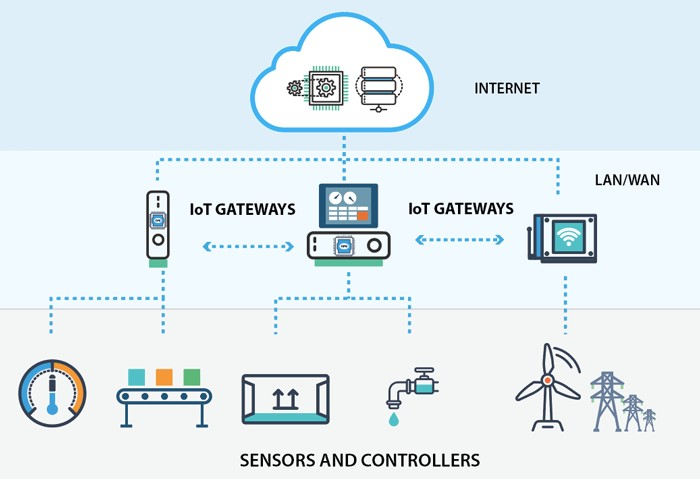
\includegraphics[scale=0.6]{figuras/architecture.jpg}
  \end{adjustbox}
  \caption{Representación gráfica de la arquitectura de SmartRural}
  \label{fig:arquitectura}
\end{figure}

\section{Implementación}
La implementación de este proyecto es una de las mejores definiciones que se podrían dar de un sistema distribuido
encargado de gestionar eventos complejos.

Así pues, empezamos a listar:

\begin{itemize}
  \item \textbf{Java y Maven:} para la generación aleatoria de los datos
        simulando la información dada por cualquier sensor.
  \item \textbf{ThingSpeak:} plataforma usada para almacenar brevemente
        la información de los sensores.
  \item \textbf{Anypoint Studio y Mule:} usado para obtener la información
        y disparar los eventos complejos que realizaran las
        distintas acciones de automatización.
  \item \textbf{Esper:} para la creación de los eventos.
  \item \textbf{MySQL:} para guardar la información después del procesamiento
        por el Mule y proveer al backend de información.
  \item \textbf{NodeJS:} usado para hacer el backend, acceder a la base de datos
        y hacer un CRUD de la misma mediante endpoints
        para proveer a un frontend que se encargue de mostrar de forma agradable la información.
  \item \textbf{Ionic con React:} por último, esta tecnología nos permite crear un frontend
        amigable con pocas líneas de código
        para hacerlo amigable, multiplataforma y bonito.
\end{itemize}

\section{Pruebas}
Las únicas pruebas realizadas del entorno han sido pruebas manuales de flujo, es decir, 
se ha probado manualmente a lanzar el generador de datos y que el flujo del anypoint los
captura con éxito y dispara los eventos.

Posteriormente, esos datos se insertan en la base de datos y por último, son tratados en
el backend y mostrados en el frontend.

\clearpage

\nocite{*}
\bibliographystyle{IEEEtran}
\bibliography{bib}

\end{document}
